\documentclass[12pt,a4paper]{report}

% Packages
\usepackage[utf8]{inputenc}
\usepackage{setspace}
\usepackage{geometry}
\usepackage{hyperref}
\usepackage{graphicx}

\usepackage{tikz}
\usetikzlibrary{arrows.meta, calc, positioning}

\tikzstyle{block} = [draw, fill=white, rectangle, 
    minimum height=3em, minimum width=6em]
\tikzstyle{sum} = [draw, fill=white, circle, node distance=1cm]
\tikzstyle{input} = [coordinate]
\tikzstyle{output} = [coordinate]
\tikzstyle{pinstyle} = [pin edge={to-,thin,black}]

\onehalfspacing
\geometry{margin=1in}

\begin{document}

% Title Page
\title{Reducing the runtime of an NP-Hard algorithm using deep learning on historical data}
\author{Christoffer Lindkvist}
\date{\today}
\maketitle

% Abstract
\begin{abstract}
    SILKSONG SOON SHAW 
\end{abstract}

% Table of Contents
\tableofcontents
\listoffigures

\chapter{Introduction}
\section{Background}
    This thesis is an extension to the Volvo Truck Assembly Line problem (?); 
    Today trucks are placed manually by management workers based solely on their own knowledge, 
    though this is not written down anywhere. 
    The algorithm in the works will using data from Volvo help place the trucks so that there are as few overlaps as possible. 
    My idea is that the algorithm can gain a faster runtime by defaulting to "safe" combinations which are already used today.
    
\section{Research Problem}
\section{Objectives}
\section{How can one intuitively visualize this problem?}
    The UI will visualize the flow of the assembly line on two axes. One per station, and one in clockcycles.

    Issues start to appearing when we start to consider how to properly communicate size in relation to time in seconds when time is measured in an arbitrary unit refered to as clockcycles.

    One clockcycle is the time it takes the theoretical product to make it from one station to the next. Hence the items must be displayed in a way that conveys that some stations take longer and shorter time to complete.

\section{The Algorithm}
\subsection{The Heuristic Approach}

The problem to properly order manufacturing assembly lines with as few overlaps as possible is an NP-Hard problem. 

The Algorithm designed to solve this problem is a heuristic solution that will be made out of a Construction Hieuristic $(C\!H)$ that produces a starting point based on pre-defined constraints, that feeds into a Meta Heuristic $(M\!H)$ that finds a better solution starting from the output of the construction heuristic and self-improving until an acceptable result is returned. 
\vspace{2em} 
\begin{figure}[ht]
    \centering

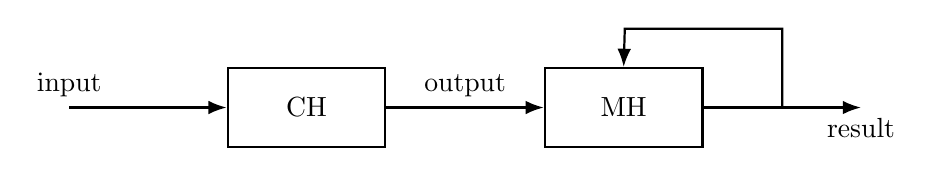
\begin{tikzpicture}[>=Latex, node distance=2cm, thick]

  \node[draw, minimum width=2cm, minimum height=1cm, align=center] (CH) {CH};
  \node[draw, minimum width=2cm, minimum height=1cm, align=center, right=of CH] (MH) {MH};

  \draw[->] ($(CH.west)+(-2,0)$) -- (CH.west) node[pos=0, above] {input};
  
  \draw[->] (CH.east) -- (MH.west) node[midway, above] {output};

  \draw[->] (MH.east) -- ++(1,0) -- ++(0,1) -- ++(-2,0) -- (MH.north);      

  \draw[->] (MH.east) -- ++(2,0) node[pos=1, below] {result};

\end{tikzpicture}
    \caption{Heuristic solution}
    \label{fig:ml_solution}
\end{figure}

\subsection{Complementing the Heuristic Approach using Machine Learning}
Due to the fact that servicemen today place products to be made manually using unwritten knowledge they have accumulated over the years.

The idea is that if they have knowledge of a good enough solution from the get-go with some risk of overlap, then we can train a Deep Learning Model $(M\!L)$ on such previous data to give the algorithm a better starting point, thus reducing the runtime of that algorithm.

\begin{figure}[ht]
    \centering
    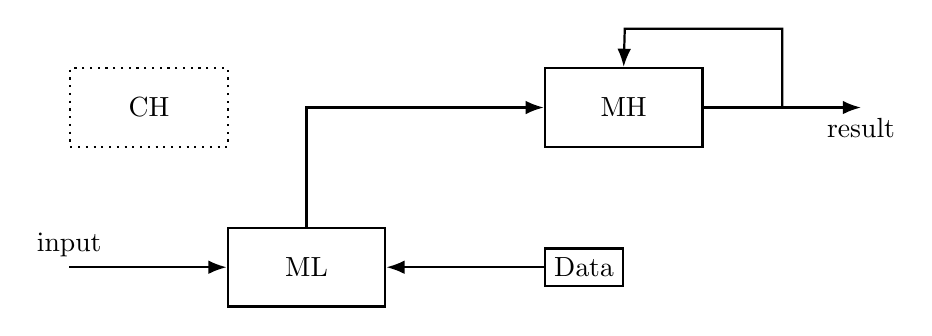
\begin{tikzpicture}[>=Latex, node distance=2cm, thick]
        \node[draw, minimum width=2cm, minimum height=1cm, align=center] (MH) {MH};
\node[draw, minimum width=2cm, minimum height=1cm, below left=1cm and 2cm of MH] (ML) {ML};
        \node[draw, align=center, right=of ML] (Data) {Data};
        \node[draw, dotted, minimum width=2cm, minimum height=1cm, align=center, left=4cm of MH] (CH) {CH};
        \draw[->] (MH.east) -- ++(1,0) -- ++(0,1) -- ++(-2,0) -- (MH.north);      

        \draw[->] (MH.east) -- ++(2,0) node[pos=1, below] {result};

        \draw[->] ($(ML.west)+(-2,0)$) -- (ML.west) node[pos=0, above] {input};

        \draw[->] (Data.west) -- (ML.east);

        \draw[->] (ML.north) |- (MH.west);

    \end{tikzpicture}
    \caption{ML solution}
    \label{fig:ml_solution}
\end{figure}


\chapter{Literature Review}
\section{Theoretical Framework}
\section{Previous Work}
\section{Research Gaps}

\chapter{Machine Learning}
\section{Why Machine Learning}
\section{Data Collection}
\section{Data Analysis}

\chapter{Results}
\section{Findings}
\section{Data Presentation}

\chapter{Discussion}
\section{Interpretation of Results}
\section{Comparison with Literature}
\section{Implications}

\chapter{Conclusion}
\section{Summary of Findings}
\section{Limitations}
\section{Future Work}

% References
\begin{thebibliography}{99}
\bibitem{ref1}
J. Abbasi, \textit{Predictive Maintenance in Industrial Machinery using Machine Learning}, 
Master’s thesis, Luleå University of Technology, Department of Computer Science, Electrical and Space Engineering, 2021.
\bibitem{ref2}
A. Dupuis, C. Dadouchi, and B. Agard, 
        \textit{A decision support system for sequencing production in the manufacturing industry},
\textit{Computers \& Industrial Engineering}, vol.~185, p.~109686, 2023. 
doi: \href{https://doi.org/10.1016/j.cie.2023.109686}{10.1016/j.cie.2023.109686}.
\bibitem{ref3} Author, Title, Journal, Year.

\end{thebibliography}

\appendix
\chapter{Appendix A}
    bruh
\end{document}
